\documentclass[]{article}
\usepackage{amsmath}\usepackage{amsfonts}
\usepackage[margin=1in,footskip=0.25in]{geometry}
\usepackage{mathtools}
\usepackage{hyperref}
\hypersetup{
    colorlinks=true,
    linkcolor=blue,
    filecolor=magenta,
    urlcolor=cyan,
}
\usepackage[final]{graphicx}
\usepackage{listings}
\usepackage{courier}
\lstset{basicstyle=\footnotesize\ttfamily,breaklines=true}

% \usepackage{wrapfig}
\graphicspath{{.}}

\begin{document}
\begin{center}
    Name: Hongda Li \quad Class: CSE 546 \quad HW2B
\end{center}
\section*{B.1}
    \textbf{Objective}: Given the definition for the L2, L1 and the Infinity norm of real vector, show that $\Vert x\Vert_\infty \le \Vert x\Vert_2 \le \Vert x\Vert_1$. 
    \\
    First we are going to show that $\Vert x\Vert_2^2 \le \Vert x\Vert_1^2$, starting from the definition of the norms we have: 
    \begin{align*}\tag{B.1.1}\label{eqn:B.1.1}
        \Vert x\Vert_1^2 &= 
            \left(
                \sum_{i = 1}^{n} |x_i|
            \right)^2
        \\ 
        &= \sum_{i = 1}^{n}
            \left(
                |x_i|\sum_{j = 1}^{n}
                    |x_j|
            \right)
        \\
        &= 
        \sum_{i = 1}^{n}
            \left(
                |x_i|^2 + 
                |x_i|\sum_{j = 1, j \ne i}^{n}
                    |x_j|
            \right)
        \\
        &= 
        \sum_{i = 1}^{n} |x_i|^2 + \sum_{i = 1}^{n}|x_i|\left(
            \sum_{ j= 1,j \ne i }^{n}
                |x_j|
        \right)
        \\
        &= 
        \Vert x\Vert_2^2 + \underbrace{\sum_{i = 2}^{n}\sum_{j = 1}^{i - 1}2|x_i||x_j|}_{\ge 0}
        \\
        &\implies \Vert x\Vert_2^2 \le \Vert x\Vert_1^2
    \end{align*}
    And now we are going to shoe that $\Vert x\Vert_\infty^2 \le \Vert x\Vert_2^2$. By the definition of the infinity norm, we know that therde exists $1\le m \le n$ such that $x_m = \Vert x\Vert_\infty = \max_{1\le i\le n}(x_i)$. Then it can be said that: 
    \begin{align*}\tag{B.1.2}\label{eqn:B.1.2}
        x_m^2 \le& x_m^2 + \underbrace{\sum_{i = 1, i\ne m}^{n} x_i^2}_{\ge 0}
        \\
        x_m^2 =& \Vert x\Vert_\infty \le \sum_{i = 1}^{n}x_i^2 = \Vert x\Vert_2^2
    \end{align*}
    And then combing together, we can take the square root because the function $\sqrt{\bullet}$ is monotone increase, hence it preserves the inequality, which will give us $\Vert x\Vert_\infty \le \Vert x\Vert_2^2\le \Vert x\Vert_1$.
\section*{B.2}
    \subsection*{B.2.a}\label{B.2.a}
        \textbf{Objective}: The function $\Vert x\Vert$ is a convex function. 
        \begin{align*}\tag{B.2.a.1}\label{eqn:B.2.a.1}
            \Vert \lambda x + (1 - \lambda)y \Vert 
            & \le \Vert \lambda x\Vert + \Vert (1 - \lambda) y\Vert
            \\
            & = \lambda\Vert  x \Vert +  (1 - \lambda)\Vert y\Vert
        \end{align*}
        Note, I just directly apply the Triangular inequality of the norm to get the inequality, and then becaues $\lambda\in[0, 1]$, so there is no absolute value, and notice that the resulting expression is the definition of Convexity the given function.   
    \subsection*{B.2.b}        
        \textbf{Objective}: Show that the set $\{x \in \mathbb{R}^n: \Vert x\Vert \le 1 \}$ is a convex set. Let the set be denoted as $S$ Let's take any 2 points in the set like $x \in S$,  $y \in s$, then $\Vert x\Vert \le 1$ and $\Vert y\Vert\le 1$ for any line defined by the 2 points: 
        \begin{align*}\tag{B.2.b.1}\label{eqn:B.2.b.1}
            \Vert \lambda x + (1 - \lambda)y \Vert &\le 
            \lambda \underbrace{\Vert x\Vert}_{\le \lambda} + \underbrace{(1 - \lambda)\Vert y\Vert}_{\le 1 - \lambda}
            \\
            \implies
            \Vert \lambda x + (1 - \lambda)y \Vert &\le 1
            \\
            \implies \lambda x + (1 - \lambda)y &\in S
        \end{align*}
        The first by the inequality of norm, and the second is by the definition of the fact that $x,y \in S$, and the third is by the definition of the set $S$.
    \subsection*{B.2.c}
        The set $ \{(x_1, x_2): g(x_1, x_2) \le 4\}$ domain of the function such that the value of the function is bounded by a given quantity. This is the unit norm ball defined by $p = \frac{1}{2}$. As we showned in lecture, it's not convex, and it looks like a star\footnote{Drawn by mathematica. }:  
        \begin{center}
            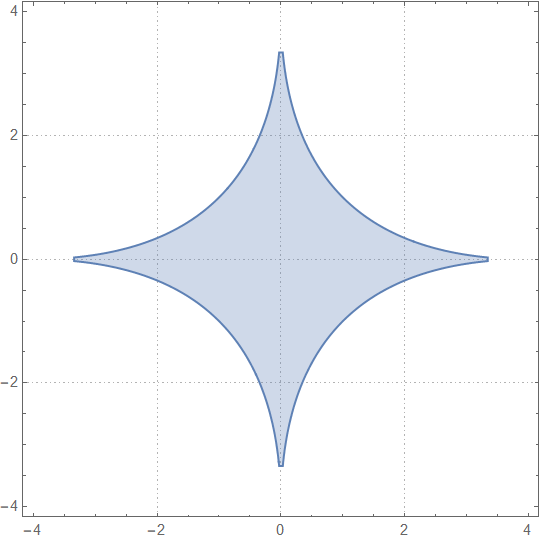
\includegraphics[width=10cm]{b2-norm-ball.png} 
        \end{center}
    
\section*{B.3}  
    \subsection*{B.3.a}
        \textbf{Objective}: Showing that, the squared loss function regularized with Eclidean norm (not squared) is convex. The trick is to show that, the squared loss function is convex, and we have shown the the Euclidean norm is convex back in \hyperref[B.2.a]{B.2.a}. And by showing that the positive weighted sum of 2 convex function is convex, we will be able to show that it's convex. 
        \\
        The loss function is convex because: $l_i(w) = (y_i - w^Tx_i)^2$, this function is qaudratic, and it's second derivative is $\text{diag}(2)$ (The hessian fof the function wrt to $w$), which is a positive quantity. When the second derivative of a function is always larger than or equals to zero, the function is convex. 
        \\
        Here, we will show that the sum of 2 convex function is convex too. Let $f(x), g(x)$ be 2 convex function mapping $x\in \mathbb{R}^n$ to $\mathbb{R}$. Choose any 2 points $x, y\in \mathbb{R}^n$ then we have: 
        \begin{align*}\tag{B.3.a.1}\label{eqn:B.3.a.1}
            f(\lambda x + (1 - \lambda)y) \le& \lambda f(x) + (1 - \lambda)f(y) 
            \\
            & \wedge
            \\
            g(\lambda x + (1 - \lambda)y) \le& \lambda g(x) + (1 - \lambda)g(y) 
            \\
            \implies 
            f(\lambda x + (1 - \lambda)y) + g(\lambda x + (1 - \lambda)y)
            &\le \lambda f(x) + (1 - \lambda)f(y) +  \lambda g(x) + (1 - \lambda)g(y) 
            \\
            f(\lambda x + (1 - \lambda)y) + g(\lambda x + (1 - \lambda)y)
            &\le
            \lambda (f(x) + g(x)) + (1 - \lambda) (f(x) + g(x))
        \end{align*}
    It's not hatd to see that, if we set $h(x) := g(x) + h(x)$ then the last line of the statement will be the convexity of $h(x)$, proving the that sume of the 2 functions are still convex. 
    \\
    \textbf{Note}: If the sum 2 functions are still convex, then \textbf{the sum finite many function is still going to be convex}, this can be proved inductively, because the $+$ sign is associatitve.  
    \\
    Using this, and using the fact that $\sum_{i = 1}^{n} l_i(w) + \lambda\Vert w\Vert$ is convex, because all the function we are summing up are convex function.
    \subsection*{B.2.b}
        Convex loss function is easier to optimize, it has minimal, and it's a convex set of minimal as well. And the use of a \textbf{strictly convex regularizer} will give \textbf{unique global optimal}, the strongly convex loss function is the best, because gradient descent performs really well on them. 
\section*{B.4: Multinomial Logistic Regression}
    \subsection*{B.4.a}
        We are going to take the gradient on the loss function. Our objective is to find the log MLE of the following Loss Function: 
        \begin{align*}\tag{B.4.1}\label{eqn:B.4.1}
            \mathcal{L}(W) = - \sum_{i = 1}^{n} \sum_{l = 1}^{k}
                \mathbf{1}\{y_i = l\} \log \left(
                    \frac{\exp \left(
                        w^{(l)}\cdot x_i
                    \right)}{
                        \sum_{j = 1}^{k}
                        \exp \left(
                            w^{j}\cdot x_i
                        \right)
                    }
                \right)
        \end{align*}
        To find the gradient of the loss function wrt the parameter matrix $W = [w^{(1)}, w^{(2)}, \cdots,w^{(k)}]$. We are going to take the gradient on the loss function wrt each column of the matrix and then we will stack then horizontal together to get the resulting matrix. Let's consider
        \begin{align*}\tag{B.4.2}\label{eqn:B.4.2}
            \nabla_{w^{(m)}}L(W) 
            &= 
            -\sum_{i = 1}^{n}
            \sum_{l = 1}^{k}
                \mathbf{1}\{y_i = l\}
                \nabla_{w^{(m)}} \left[
                    \log \left(
                    \frac{x_i^T\exp(x_i^Tw^{(l)})}{
                        \sum_{j = 1}^{k}
                            \exp(x_i^T w^{(j)})
                    }
                    \right)
                \right]
        \end{align*}
        Let's take a look at the inner part more carefully, and simpifying it will give us something like: 
        \begin{align*}\tag{B.4.3}\label{eqn:B.4.3}
            \nabla_{w^{(m)}} \left[
                \log \left(
                \frac{x_i^T\exp(x_i^T w^{(l)})}{
                    \sum_{j = 1}^{k}
                        \exp(x_i^T w^{(j)})
                }
                \right)
            \right] &= 
            \left(
                \begin{cases}
                    x_i  & l = m 
                    \\
                    0 & \text{else}      
                \end{cases}
            \right)
            -
            \partial_{w^{(m)}}\left[
                \log
                \left(
                    \sum_{j = 1}^{k}
                        \exp\left(
                            x_i^T w^{(j)}
                        \right)
                \right)
            \right]
            \\
            &=
            \left(
                \begin{cases}
                    x_i  & l = m 
                    \\
                    0 & \text{else}      
                \end{cases}
            \right)
            -
            \frac{
                \partial_{w^{(m)}} \left[
                    \sum_{j = 1}^{k}
                        \exp\left(
                            x_i^T w^{(j)}
                        \right)
                \right]
            }{
                    \sum_{j = 1}^{k}
                        \exp\left(
                            x_i^T w^{(j)}
                        \right)
            }
            \\
            &=
            \left(
                \begin{cases}
                    x_i  & l = m 
                    \\
                    0 & \text{else}      
                \end{cases}
            \right)
            -
            \frac{
                \exp(x_i^T w^{(m)})x_i
            }{
            \sum_{j = 1}^{k}
                \exp\left(
                    x_i^T w^{(j)}
                \right)
            }
            \\
            &= 
            x_i\left(
                \mathbf{1}\{l = m\} - 
                \frac{
                    \exp(x_i^T w^{(m)})x_i
                }{
                \sum_{j = 1}^{k}
                    \exp\left(
                        x_i^T w^{(j)}
                    \right)
                }
            \right)
        \end{align*}
        Do take note that $l = m \iff y_i = l$ and these 2 evets happens at the same time and they are interchangable.  
        \\
        And we follow the tradition of using the label vector from previous HW1, which is that each of the $y_i$ is a column vector, and it's $1$ in the ``i'' th position of the vector, denoting the the data $x_i$ has label $i$. 
        \\
        Another thing we are going to make use is the $\text{softmax}(\theta)$ which is a vector function mapping from $\mathbb{R}^k$ to $\mathbb{R}^k$: 
        $$
            \left(
                \text{softmax}(\theta)
            \right)_m
            = \frac{\exp(\theta_m)}{
                \sum_{j = 1}^{k}\exp(\theta_j)
            }
        $$
        Where, we showcase the $m$ th element of this function when we put into the vector $\theta$. 
        \\
        We may use this to simply simpify the cases situation above, and that should give us: 
        \begin{align*}\tag{B.4.4}\label{eqn:B.4.4}
            -\sum_{i = 1}^{n}
                \mathbf{1}\{y_i = l\}
                \nabla_{w^{(m)}} \left[
                    \log \left(
                    \frac{x_i^T\exp(x_i^T w^{(l)})}{
                        \sum_{j = 1}^{k}
                            \exp(x_i^T w^{(j)})
                    }
                    \right)
                \right] 
            &= 
            -\sum_{i = 1}^{n} 
            x_i \left(
                \mathbf{1}\{y_i = l\} - 
                \underbrace{\frac{
                        \exp(x_i^T w^{(m)})
                    }{
                            \sum_{j = 1}^{k}
                                \exp\left(
                                    x_i^T w^{(j)}
                                \right)
                   }}_{(\text{softmax}((x_i^TW)^T))_m}
                \right)
            \\
            &= 
            -\sum_{i = 1}^{n} 
            x_i \left(
                \mathbf{1}\{y_i = l\}
                - (\text{softmax}(W^Tx_i))_m
                \right)
        \end{align*}
        Now, I am going horizontally stack all these vector together, and notice that it can be written as an outter product, and the condition $\mathbf{1}(y_i = l)$ can be replaced with the appropriate label vector $y_i$, and this will be like: 
        \begin{align*}\tag{B.4.5}\label{eqn:B.4.5}
            \nabla_{W}\mathcal{L}(W) &=
            -\sum_{i = 1}^{n}
                x_i(y_i - \text{softmax}(W^Tx_i))^T
        \end{align*}
        Then in this case, we just need to make the definition that: 
        $$
            \hat{y}_i^{W} = \text{sfotmax}(W^Tx_i)
        $$
        Then substituting this back to the previous part, we have the expression that: 
        \begin{align*}\tag{B.4.6}\label{eqn:B.4.6}
            \nabla_{W}\mathcal{L}(W) &=
            -\sum_{i = 1}^{n}
                x_i(y_i - \hat{y}_i^{(W)})^T
        \end{align*}
    \subsection*{B.4.b}
    
\section*{B.5: Confidence Interval of Least Squares Estimation: Bounding Estimate}


\end{document}
